\documentclass[10pt,a4paper,twoside]{article}
\usepackage[english]{babel}
%laad de pakketten nodig om wiskunde weer te geven :
\usepackage{amsmath,amssymb,amsfonts,textcomp}
%laad de pakketten voor figuren :
\usepackage{graphicx}
\usepackage{float,flafter}
\usepackage{hyperref}
\usepackage{inputenc}
\usepackage{minted}
\usepackage{subcaption}

\setlength\paperwidth{20.999cm}\setlength\paperheight{29.699cm}\setlength\voffset{-1in}\setlength\hoffset{-1in}\setlength\topmargin{1.499cm}\setlength\headheight{12pt}\setlength\headsep{0cm}\setlength\footskip{1.131cm}\setlength\textheight{25cm}\setlength\oddsidemargin{2.499cm}\setlength\textwidth{15.999cm}

\newcommand{\sweepsize}{0.26}

\begin{document}
\begin{center}
\hrule

\vspace{.4cm}
{\bf {\Huge Computer Vision} \\ {\huge Lab Assigment Report} \\ {\Large Object recognition}}
\vspace{.2cm}
\end{center}
{\bf Tuan Mate Nguyen}  (tunguyen@student.ethz.ch)
\hrule



\section{Bag-of-Words classifier}
\subsection{Local feature extraction}
First for both dimension I createad the coordinate points using numpy's linspace.
These are floating point numbers as the borderless dimensions might not be
divisible by the number of points. Also it's always a good idea to check if
input parameters make sense.

\begin{minted}[mathescape,
    linenos,
    numbersep=5pt,
    gobble=2,
    frame=lines,
    framesep=2mm,
    firstnumber=47]{csharp}
    assert(2*border<h)
    assert(2*border<w)
    grid_coord_y = np.linspace(border, h-border-1, nPointsY)
    grid_coord_x = np.linspace(border, w-border-1, nPointsX)
\end{minted}



All possible pairs of these coordinates -
given by meshgrid() - define the points of the grid. 

\begin{minted}[mathescape,
    linenos,
    numbersep=5pt,
    gobble=2,
    frame=lines,
    framesep=2mm,
    firstnumber=53]{csharp}
    grid_x, grid_y = np.meshgrid(grid_coord_x, grid_coord_y, indexing='ij')
\end{minted}

The result is transposed since the
returned array's shape must be (N,2), not (2, N).

\begin{minted}[mathescape,
    linenos,
    numbersep=5pt,
    gobble=2,
    frame=lines,
    framesep=2mm,
    firstnumber=56]{csharp}
    vPoints = np.array([grid_x, grid_y]).transpose()
\end{minted}

For the histogram, first the angles need to be computed. The gradients of
interest in the cell are extracted using the cell's four corner point. The
angles can be obtained by providing the gradient values in the $y$ and $x$
direction to numpy's arctan2(). The arctan2 function is needed so that angles
from all 4 quadrants are distinguished correctly.

\begin{minted}[mathescape,
    linenos,
    numbersep=5pt,
    gobble=2,
    frame=lines,
    framesep=2mm,
    firstnumber=86]{csharp}
                cell_grad_x = grad_x[start_y:end_y, start_x:end_x]
                cell_grad_y = grad_y[start_y:end_y, start_x:end_x]
                angles = np.arctan2(cell_grad_y, cell_grad_x)
\end{minted}

The flattened values are then fed to the histogram generator function. The bin
edges are ignored.

\begin{minted}[mathescape,
    linenos,
    numbersep=5pt,
    gobble=2,
    frame=lines,
    framesep=2mm,
    firstnumber=90]{csharp}
                hist, _ = np.histogram(angles.flatten(), nBins, (-np.pi, np.pi))
\end{minted}

\subsection{Codebook construction}
In order to create the codebook, the previous functions are just chained
together. The result is the input to the k-means algorithm.

\begin{minted}[mathescape,
    linenos,
    numbersep=5pt,
    gobble=2,
    frame=lines,
    framesep=2mm,
    firstnumber=128]{csharp}
        vPoints = grid_points(img, nPointsX, nPointsY, border)
        descriptors = descriptors_hog(img, vPoints, cellWidth, cellHeight)
\end{minted}


\subsection{Bag-of-Words vector encoding}
For the vector encoding, for each input feature vector the closest center's index
need to be determined using the provided findd() function. The number of centers
is the first dimension of the center array. Only the count of indices
are interesting so the distances are ignored. Then the occurrences of each center
index can be counted, constructing the BoW histogram.

\begin{minted}[mathescape,
    linenos,
    numbersep=5pt,
    gobble=2,
    frame=lines,
    framesep=2mm,
    firstnumber=153]{csharp}
    nClusters = vCenters.shape[0]
    idx, _ = findnn(vFeatures, vCenters)
    histo = np.bincount(np.array(idx), minlength=nClusters)
\end{minted}

When processing the training examples, I created the feature vector for each of
them and then passed them to the BoW histogram constructor. The result is a
signature histogram - with respect to the codebook's words - for each image.
This step is repeated for positive and negative examples.

\begin{minted}[mathescape,
    linenos,
    numbersep=5pt,
    gobble=2,
    frame=lines,
    framesep=2mm,
    firstnumber=185]{csharp}
        vPoints = grid_points(img, nPointsX, nPointsY, border)
        vFeatures = descriptors_hog(img, vPoints, cellWidth, cellHeight)
        vBoW.append(bow_histogram(vFeatures, vCenters))
\end{minted}

\subsection{Nearest neighbor classification}
To classify a test image, I checked the test image's histogram's distance to
that of the training samples, once again using the findnn() function, this time
discarding the matching image's index, only caring about the distance (first
element of the returned 1-element list).

The label of the closer one of the closest positive and negative neighbor will be
assigned to the test image.

\begin{minted}[mathescape,
    linenos,
    numbersep=5pt,
    gobble=2,
    frame=lines,
    framesep=2mm,
    firstnumber=205]{csharp}
    _, DistPoss = findnn(histogram, vBoWPos)
    _, DistNegs = findnn(histogram, vBoWNeg)
    DistPos = DistPoss[0]
    DistNeg = DistNegs[0]
\end{minted}

\subsection{Results}
Using $k=12$ and $numiter=200$ achieved $96\%$ accuracy both for the positive
and negative test examples. For fewer clusters the histograms of positive and
negative training examples are not distinctive enough. For more, probably there
would need to be more feature points. Increasing the number of iterations will
stop improving the accuracy after a point.


\section{CNN-based classifier}
\subsection{Simplified version of VGG network}
The simplified VGG network consists of 5 convolutional layer and one fully
connected layer. The convolutional layers are similar, all having a ReLU
activation function and a max pooling added. The output of the last
convolutional layer is a $batch\_size \times 512 \times 
1 \times 1$ array, which needs
to be reshaped into a $batch\_size \times 512$ array to be compatible with the
fully connected layer's $512 \times \# fc\_layer$ shape.

The output has $batch\_size \times \# classes$ shape.

\begin{minted}[mathescape,
    linenos,
    numbersep=5pt,
    gobble=2,
    frame=lines,
    framesep=2mm,
    firstnumber=80]{csharp}
        y = self.conv_block1(x)
        y = self.conv_block2(y)
        y = self.conv_block3(y)
        y = self.conv_block4(y)
        y = self.conv_block5(y)
        y = y.view(-1, 512)
        score = self.classifier(y)
\end{minted}


\subsection{Training and testing}
For training I used a batch size of 128 and 50 epochs. I haven't done too much
experimenting as the runtime of the training was almost 4 hours. As Fig.\ref{result}
shows, the loss decreases and the accuracy increases during training, both
reaching a plateau as expected. The achieved
accuracy on the test set was $81.57\%$.

\begin{figure}[h]
    \centering
    
    \begin{subfigure}{0.4\textwidth}
    \includegraphics[width=\linewidth]{training_loss.png} 
    \caption{Training loss}
    \end{subfigure}
    \begin{subfigure}{0.4\textwidth}
    \includegraphics[width=\linewidth]{training_acc.png} 
    \caption{Validation accuracy}
    \end{subfigure}
    \caption{Training loss and validation accuracy over the course of training}

    \label{result}
\end{figure}
% Python code
%\begin{minted}[mathescape,
%    linenos,
%    numbersep=5pt,
%    gobble=2,
%    frame=lines,
%    framesep=2mm,
%    firstnumber=26]{csharp}
%\end{minted}

% Image
%\begin{figure}[H]
%    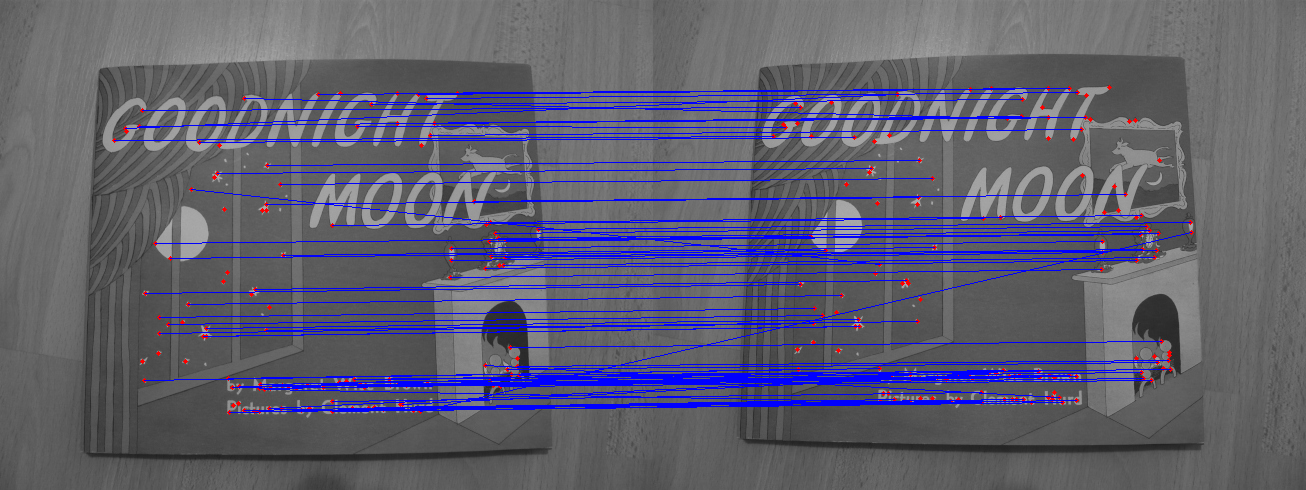
\includegraphics[width=\textwidth]{match_mutual.png}
%    \centering
%    \caption{Matching keypoints for mutual nearest neighbor matching}
%    \label{match_mutual}
%\end{figure}

\end{document}
